% !TEX root = ../zenkoku.tex
\section{結果}

理解度は値が高いほど理解が深いものとし,`熟練者の理解度 - 熟練者を除いた回答者の理解度平均` によって求めた数値を熟練者への依存度の高さとする.
縦軸がブルーム・タキソノミーでの理解度,横軸が設問カテゴリ(各サブシステム)となっている.
また重ね合わせられている棒グラフは熟練者への依存度の高さを表している.

結果を\ri{img:rikai}に示す.

\begin{figure}[t]
	\centering
	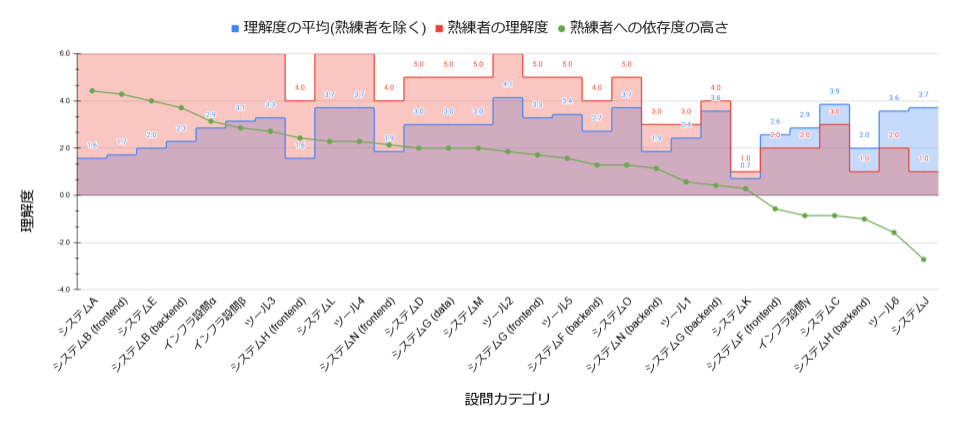
\includegraphics[keepaspectratio,width=0.9\linewidth]{img/rikai.png}
	\caption{理解度の平均と熟練者への依存度の高さ}
	\label{img:rikai}
\end{figure}
